\documentclass[12pt,twoside]{article}
\usepackage{setspace,epsfig,multicol,fancyhdr,amssymb,amsmath,amsfonts,lastpage,array,stmaryrd,color,graphics,multicol,wrapfig,graphicx,hhline,lineno,textcase,pifont,textcomp,ragged2e,url,nextpage}
\usepackage[normalem]{ulem}
\usepackage[utf8]{inputenc}

%\psdraft
\graphicspath{{./figures/}}
\input{/home/pisti/programs/latex/styles/color_defs}
fj/preamble.tex

%%%% Firdaus'


%%%% for ARIAL font (helvetica)
% \renewcommand{\familydefault}{\sfdefault}
%\renewcommand{\rmdefault}{phv} % Arial
%\renewcommand{\sfdefault}{phv} % Arial

% characters utf8 : ••••••••••••••••••••••••••••• • 
	
\setstretch{1}
\textwidth 160mm
\topmargin -18mm
\textheight 250mm
%\textheight 260mm
\headheight 14pt
\oddsidemargin 5mm
\evensidemargin 5mm
\marginparwidth 25mm
\marginparsep 3mm
\marginparpush 0in
%\footskip 0mm
 
\pagenumbering{arabic}

%%%% for bibliography
%\usepackage{natbib}		% see petek.html, #BibTeX
\usepackage[super,comma,sort&compress]{natbib}
\renewcommand{\cite}[1]{{\color{blue}\citep{#1}}}
%\newcommand{\CITE}[1]{{\color{citeblue}\citep{#1}}}

%%%% in order to avoid square brackets in citation list reference 
\makeatletter
\def\@cite#1#2{({#1\if@tempswa , #2\fi})}
\def\@biblabel#1{#1.}
\makeatother

\setstretch{1}

\renewcommand{\thefootnote}{\color{red}{\fnsymbol{footnote}}}
\renewcommand{\headrulewidth}{.4pt}

\newcommand{\myParagraph}[1]{
  \addtocounter{paragraph}{1}
  \paragraph{\textbf{\Alph{section}.\arabic{subsection}.\arabic{subsubsection}.\arabic{paragraph}} {#1}}}

\newcommand\ttt[1]{{\color{studyblue}\textup{\ttfamily\normalsize #1}}}
\newcommand{\myBlue}{\noindent{\color{studyblue}{\large\bf\textsf{\myStr\ }}}}
\newcommand{\myblue}{\noindent{\color{studyblue}{\myStr}}}
\newcommand{\myRed}{\noindent{\color{darkred}{\bf\myStr}}}
\newcommand{\myred}{\noindent{\color{darkred}{\myStr}}}
\newcommand{\HMM}{{\color{darkred}\textbf{\textsf{HMM\ }}}}

\begin{document} %%%%%%%%%%%%%%%%%%%%%%%%%%%%%%%%%%%%%%%%%%%%%%%%%%%%%%%%%%%%%%%%%%%%%%%%%%%%%%%%%%%

%\enlargethispage{1cm}
%\thispagestyle{empty}
\pagestyle{empty}
\pagenumbering{arabic}
\setcounter{page}{1}

%\noindent\hspace{-10mm}\makebox[0mm][l]{\raisebox{-245mm}[0mm][0mm]{\colorbox{gray}{\rule{183mm}{0mm}\rule{0mm}{246mm}}}}
\noindent\hspace{-10mm}\makebox[0mm][l]{\raisebox{-238mm}[0mm][0mm]{\colorbox{graygreen}{\rule{183mm}{0mm}\rule{0mm}{246mm}}}}
%\vspace*{5mm}

\begin{spacing}{2}
\noindent\scalebox{2.3}{\parbox{70mm}{\textbf{\textsf{\center\Huge{{\color{studyblue}\textbf{User Manual}}\newline \rule{0mm}{3ex}\HMM \newline\rule{0mm}{3ex}Spatio--Temporal\newline State--Space\newline Analysis\newline for fMRI}}}}}
\end{spacing}

\vspace{22mm}

\newcommand{\myVersion}{v0.04}
\begin{spacing}{1.5}
  {\large\noindent \today\\  {\color{studyblue}\textbf{User Manual (\myVersion) -- to use with fMRI data}}\\ Firdaus Janoos, Ph.D., and István Ákos Mórocz\,, M.D., Ph.D.}
\end{spacing}

%\vspace{-30mm}

%%%% that's actually for next page #2
\textheight 230mm

%\cleartoevenpage\thispagestyle{empty}\rule{0mm}{0mm}
%\cleartooddpage\thispagestyle{empty}\rule{0mm}{0mm}

\cleartooddpage\pagestyle{empty}\rule{0mm}{0mm}

%%%%%%%%%%%%%%%%%%%%%%%%%%%%%%%%%%%%%%%%%%%%%%%%%%%%%%%%%%%%%%%%%%%%%%%%%%%%%%%%%%%%%%%%%%%%%%%%%%%%

%%%% header and footer for the coming pages
\pagestyle{fancy}
\renewcommand\headrulewidth{.5pt}
\renewcommand\footrulewidth{0pt}
\fancyhead{}
\fancyfoot{}
\fancyhead[LO]{\small\HMM -- \emph{manual \myVersion}}
\fancyhead[RE]{\small\emph{manual \myVersion} -- \HMM}
\fancyhead[RO,LE]{\textsf{\small{\textbf{\color{studyblue}\thepage/\pageref{LastPage}}}}}

\tableofcontents

\cleartooddpage

%%%%%%%%%%%%%%%%%%%%%%%%%%%%%%%%%%%%%%%%%%%%%%%%%%%%%%%%%%%%%%%%%%%%%%%%%%%%%%%%%%%%%%%%%%%%%%%%%%%%

% grep "cite{" fj/*tex | cut -d "{" -f 2 | cut -d "}" -f 1 | sort | uniq
%
% Alexander2000
% Bellec2010
% Ibanez2003
% Janoos2010g
% Janoos2010g,Janoos2011
% Janoos2011
% Patel2006
% TheFILMethodsGroup2011

This manual describes the procedure for building and analyzing
spatio-temporal state-space models of neural processes.  Please refer
to \cite{Janoos2011}.  A flowchart depiction of the algorithm
developed in that paper is shown in \Fig{fig:pipeline}

\begin{figure}[h!]
\centering {
  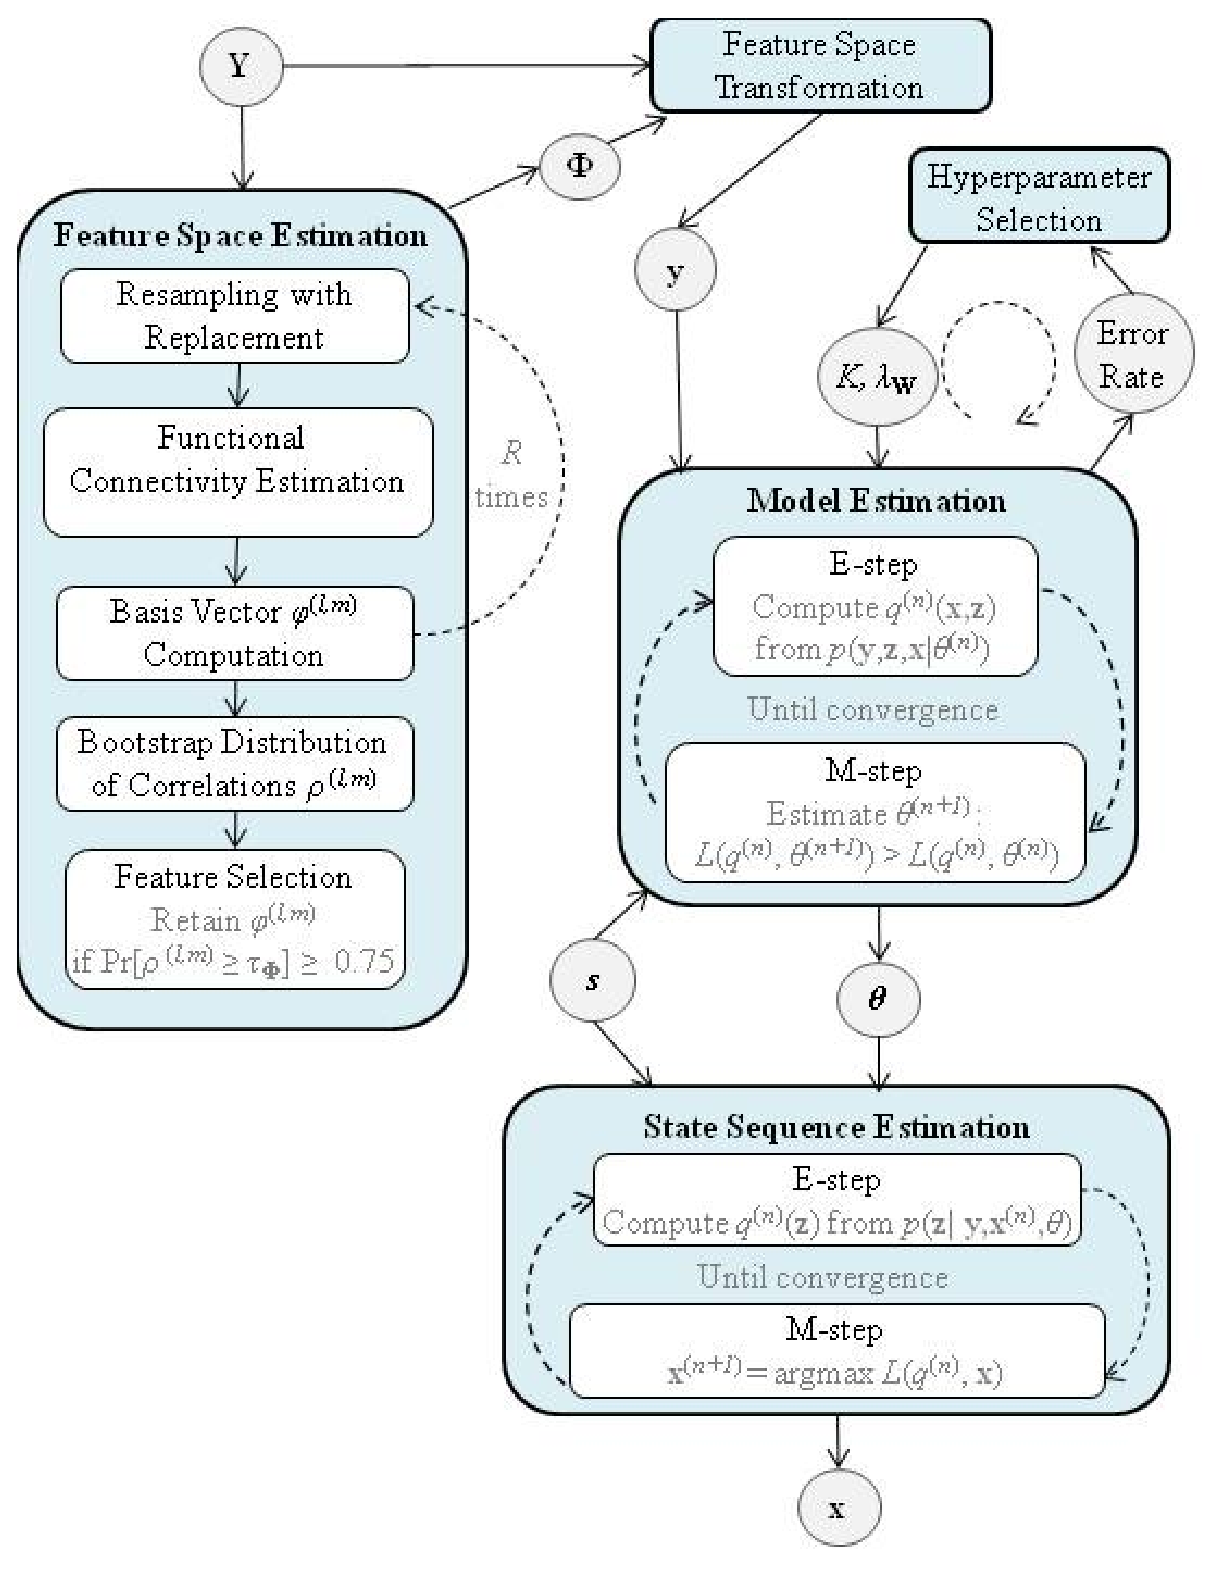
\includegraphics[width=0.8\linewidth]{pipeline-v2}}
  \caption[Outline of Method]{
  Basis vectors of the feature--space $\Phi$ are computed from the functional
  connectivity of the brain estimated from
  the fMRI data $\y$.  Dimensionality reduction is performed
  by retaining stable basis vectors using bootstrapping.
  The data ($\Y$), after projecting into the low dimensional feature--space
 are used to estimate model   parameters $\theta$ through a
  generalized EM algorithm.
  Model hyper--parameters $K$ and $\lambda_\w$ are selected
  to minimize the error of predicting the stimulus $\s$.
  Given a set of model parameters, the optimal
  state--sequence $\X^*$ is estimated using EM.
  }\label{fig:pipeline}
\end{figure}

This algorithm has been implemented in a combination of
MATLAB$^\circledR$ codes, MATLAB$^\circledR$ with
Star-P$^\circledR$, and \verb"C++".

\section{Single Session Analysis}
The main steps involved in analyzing a single session\footnote{That
is, to analyze one continuous fMRI time-series of one subject, one
session. It may consists of one actual run, or multiples runs
concatenated together. Essentially, one session is any fMRI
time-series that shares the same anatomy and imaging
characteristics.} data-set are:
\begin{enumerate}[i]
  \item Preprocessing for
  \begin{enumerate}
    \item Slice timing correction
    \item Head motion correction
    \item De-noising
    \item Head motion artifact removal
    \item Other signal artifact removal (e.g. scanner drift, pulsatile signal, respiratory signal)
  \end{enumerate}
  \item Building the feature space
  \item Specifying the experimental design
  \item Model estimation
  \item Model exploration
\end{enumerate}

\section{Multi-Subject Analysis}
In addition to the steps required for a single session analysis,
during the preprocessing step  data is spatially normalized into a
reference coordinate system using non-linear registration.

Group level analysis is performed by comparing the models across
subjects, in terms of state-space behavior and spatial activation
patterns.

\section{Prerequisites}

\subsection{Hardware}
A really fast computer / workstation to examine and explore the
results. Access to a kick-ass cluster to do the heavy duty
computation.

\subsection{Software}
\begin{enumerate}
  \item MATLAB$^\circledR$ on the work-station for design
  specification and results exploration.
  \item MATLAB$^\circledR$ with Star-P$^\circledR$ installed and
  configured, for feature-space computation and model estimation.
  \item SPM~\cite{TheFILMethodsGroup2011} version 5 or higher
  \item Group ICA of fMRI Toolbox (GIFT) \footnote{\url{http://icatb.sourceforge.net/gift}} version 1.2 or higher.
  \item An ISO Standard compatible C++ compiler.
  \item ITK\cite{Ibanez2003} version 2 or higher, installed and configured.
\end{enumerate}














\newpage








\enlargethispage{13mm}

\vspace*{-6mm}

\addcontentsline{toc}{section}{Abstract}

\section*{\scalebox{2}{\Huge{{\color{studyblue}Manual\,:} \HMM}}}

\vspace{4mm}

\begin{spacing}{1.25}

{\textsf{Abstract\,:}}\footnote{Abstract adapted from manuscript,
  \emph{in print} NeuroImage 2011} Understanding the highly complex,
spatially distributed and temporally organized phenomena entailed by
mental processes using functional MRI is an important research problem
in cognitive and clinical neuroscience. Conventional analysis methods
focus on the spatial dimension of the data discarding the information
about brain function contained in the temporal dimension. This paper
presents a fully spatio–temporal multivariate analysis method using a
state–space model (SSM) for brain function that yields not only
spatial maps of activity but also its temporal structure along with
spatially varying estimates of the hemodynamic response. Efficient
algorithms for estimating the parameters along with quantitative
validations are given. A novel lowdimensional feature–space for
representing the data, based on a formal definition of functional
similarity, is derived. Quantitative validation of the model and the
estimation algorithms is provided with a simulation study. Using a
real fMRI study for mental arithmetic, the ability of this
neurophysiologically inspired model to represent the spatio–temporal
information corresponding to mental processes is demonstrated.
Moreover, by comparing the models across multiple subjects, natural
patterns in mental processes organized according to different mental
abilities are revealed.

\end{spacing}

\vfill

\noindent\epsfig{figure=/home/pisti/munka/papers/afacan_onur/3D-EPI/figures/manuscript_fig4.eps,width=90mm}\hfill\parbox[b]{30mm}{
  \small\textsf{\textbf{Fig\,1.} Images from a heal\-thy volunteer
    acquired using a) standard 2D EPI (TR=3\,s), b) multishot 3D-EPI
    (TR=3\,s) and {\color{studyblue}c) accelerated multi- shot \HMM
      (TR=1.02\,s)}. Top row\,: axial images, middle row\,: coro\-nal
    images, bottom row\,: sagittal
    images.\\ \rule{0mm}{10mm}}}\rule{10mm}{0mm}

\vfill


\newpage

\noindent\epsfig{figure=/home/pisti/munka/papers/afacan_onur/3D-EPI/figures/new3fir.eps,width=75mm}\epsfig{figure=/home/pisti/munka/papers/afacan_onur/3D-EPI/figures/new1fir.eps,width=75mm}

\noindent\parbox[b]{160mm}{\small\textsf{\textbf{Fig\,2.} SPM results
    showing the FIR analysis (Auditory Regressor) for the
    event-related multiplication task using: (Left) multi-shot 3D EPI
    (TR=3.0\,s) and (Right) {\color{studyblue}accelerated \HMM
      (TR=1.02\,s)}. For each sequence, FIR bins corresponding to
    areas related to auditory input, number recognition and button
    press are plotted along time.}}

\begin{spacing}{1}


%%%%%%%%%%%%%%%%%%%%%%%%%%%%%%%%%%%%%%%%%%%%%%%%%%%%%%%%%%%%%%%%%%%%%%%%%%%%%%%%%%%%%%%%%%%%%%%%%%%%

\fancyhead[RO]{data acquisition -- \textsf{\small{\textbf{\color{studyblue}\thepage/\pageref{LastPage}}}}}
\fancyhead[LE]{\textsf{\small{\textbf{\color{studyblue}\thepage/\pageref{LastPage}}}} -- data acquisition}

\section{Instructions for running the \HMM sequence}


\end{spacing}



%%%%%%%%%%%%%%%%%%%%%%%%%%%%%%%%%%%%%%%%%%%%%%%%%%%%%%%%%%%%%%%%%%%%%%%%%%%%%%%%%%%%%%%%%%%%%%%%%%%%

\newpage

\cleartooddpage\rule{0mm}{0mm}
\fancyhead[RO]{\textsf{\small{\textbf{\color{studyblue}\thepage/\pageref{LastPage}}}}}
\fancyhead[LE]{\textsf{\small{\textbf{\color{studyblue}\thepage/\pageref{LastPage}}}}}
\cleartooddpage

\end{document}


















%%%%%%%%%%%%%%%%%%%%%%%%%%%%%%%%%%%%%%%%%%%%%%%%%%%%%%%%%%%%%%%%%%%%%%%%%%%%%%%%%%%%%%%%%%%%%%%%%%%%

\fancyhead[RO]{data acquisition -- \textsf{\small{\textbf{\color{studyblue}\thepage/\pageref{LastPage}}}}}
\fancyhead[LE]{\textsf{\small{\textbf{\color{studyblue}\thepage/\pageref{LastPage}}}} -- data acquisition}

\section{Instructions for running the \EPI sequence}

\begin{enumerate}
  
\item Start by selecting a new patient and then enter patient details
  as you would in a standard MRI exam. Make sure that \ttt{Research
    Mode} is selected.\\
  
  001 \epsfig{figure=../figures/3DEPI.001.eps,width=50mm}\\

 
\item From the \ttt{Patient Protocols} window select \ttt{Other} and
  then select \ttt{350-NUMBRA Human v0}.  This protocol number varies
  between scanners.\\

  002 \epsfig{figure=../figures/3DEPI.002.eps,width=68.5mm}
   

\newpage
   
\item From the list of \ttt{Series} please select the following
  sequences (use the \ttt{Ctrl}-key for adding lines) and press
  \ttt{Accept}:
  
  \begin{itemize}

  \item \ttt{1-3p Localizer} (on first line)
    
  \item \ttt{15-prescan 3D EPI}
    
  \item \ttt{16-full 3D EPI}
    
  \item \ttt{17 accelerated \EPI}
    
  \end{itemize}

\hfill\raisebox{-10mm}[0mm][20mm]{003
  \epsfig{figure=../figures/3DEPI.003.eps,width=42.2mm}}

\item After the sequences are loaded, select first the \ttt{3p
  Localizer} sequence from the lower left \ttt{Rx Manager} menu and
  press \ttt{View Edit}.\\
  
  004 \epsfig{figure=../figures/3DEPI.004.eps,width=25.6mm}
  005 \epsfig{figure=../figures/3DEPI.005.eps,width=102.4mm}\\
  

\item Press \ttt{Save Series}, \ttt{Download} and \ttt{Scan} in order
  to start the 3p-Localizer.\\

  006 \epsfig{figure=../figures/3DEPI.006.eps,width=102.4mm}
   

\newpage

\item After the 3p-Localizer is scanned, chose \ttt{prescan-3D EPI}
  from the \ttt{Rx Manager}, press \ttt{View Edit}, and open the
  \ttt{Graphic Rx} window (see fig.\,005).  Click at the center of the
  upper left image.\\

  007 \epsfig{figure=../figures/3DEPI.007.eps,width=25.6mm}
  008 \epsfig{figure=../figures/3DEPI.008.eps,width=102.4mm}\\

  
\item Close \ttt{Graphic Rx} window and click on \ttt{X}.\\

  009 \epsfig{figure=../figures/3DEPI.009.eps,width=102.4mm}\\

   
\newpage
   
\enlargethispage{10mm}
   
\item Press \ttt{Save Series}, \ttt{Download} and \ttt{Scan} in order to
  start the prescan-3D EPI.\\

  010 \epsfig{figure=../figures/3DEPI.010.eps,width=102.4mm}\\

%  011 \epsfig{figure=../figures/3DEPI.011.eps,width=102.4mm}
   

\item From the Rx menu, select \ttt{\uline{full-3D EPI}}.
  Alternatively, if you want to scan at a $3 \times$ accelerated pace,
  select \ttt{\uline{accelerated-\EPI}} instead of the full-3D EPI.
  All further instructions in this manual are identical for both
  sequence versions.\\

  012 \epsfig{figure=../figures/3DEPI.012.eps,width=25.6mm}
  013 \epsfig{figure=../figures/3DEPI.013.eps,width=25.6mm}\\


\item Press \ttt{View Edit}, open Open \ttt{Graphic Rx} menu, and
  click at the center of the upper left image.\\

  \hspace{-39mm}
  \makebox[0mm][l]{
  \epsfig{figure=../figures/3DEPI.014.eps,width=102.4mm}
  \epsfig{figure=../figures/3DEPI.015.eps,width=102.4mm}}

  014 015 


\newpage
   
\item Type 50 under \ttt{\# of Slices}.  Then move the 50-slice-slab
  into the desired brain region (in all three planes) just like you
  would do it for a 2D-EPI sequence.\\

  \hspace{-39mm}
  \makebox[0mm][l]{
  \epsfig{figure=../figures/3DEPI.016.eps,width=102.4mm}
  \epsfig{figure=../figures/3DEPI.017.eps,width=102.4mm}}

  016 017\\


\item Close \ttt{Graphic Rx} (click in \ttt{X}) and open the
  \ttt{Multi-Phase} window from the \ttt{Additional Para\-meters}
  screen.\\

  018 \epsfig{figure=../figures/3DEPI.018.eps,width=102.4mm}


\newpage

\item Select the number of volumes or \ttt{Phases per Location} and
  then press enter. Check scan length under \ttt{Total time} \,!  For
  example 18 volumes (phases) result in 54\,s scan time in the case of
  the \emph{full}-3D-EPI mode while the \emph{accelerated}-\EPI will
  show 19\,s (approx.).  Then hit the \ttt{Accept} button.\\

  019 \epsfig{figure=../figures/3DEPI.019.eps,width=67mm}
  020 \epsfig{figure=../figures/3DEPI.020.eps,width=67mm}

  031 \epsfig{figure=../figures/3DEPI.031.eps,width=67mm} (accelerated)\\

   
\item If the desired number of volumes is above 500, you need to use
  the \ttt{NEX} option to scan. For example if you want to scan 1000
  images select 500 using the Multi-Phase screen, close the
  Multi-Phase screen and then click on \ttt{NEX} option on the right
  side of the screen (see fig.\,018) and then set it to 2. This way
  the sequence will produce 1000 images.


\item Click \ttt{Save Series} and \ttt{Download}, but this time
  \uline{instead of Scan} please hit \ttt{Manual Prescan}.\\

  021 \epsfig{figure=../figures/3DEPI.021.eps,width=102.4mm} (full)

  032 \epsfig{figure=../figures/3DEPI.032.eps,width=102.4mm} (accelerated)


\newpage

\item After the \ttt{Manual Prescan} window pops up, wait a few
  clicks, then hit \ttt{Done}.\\

  022 \epsfig{figure=../figures/3DEPI.022.eps,width=81mm}\\
   

\item Now you need to start for each scan an \textbf{RDS client} that
  will read and store the raw data.  To do that you
  need to open a UNIX command window.  For that you will open a
  command window by \ttt{right click} on the blue screen background
  and select \ttt{Service Tools---Command Window} from the list of
  options.\\

  023 \epsfig{figure=../figures/3DEPI.023.eps,width=51.3mm}\\
   

\item Type in the command window\,: \ttt{cd /usr/g/research/onur/rds}
  and hit \ttt{enter}.\\

  024 \epsfig{figure=../figures/3DEPI.024.eps,width=51.3mm}
  

\newpage

\item Then type\,: \ttt{readdata exam\# series\# acquisition\#}

  For example, if your exam number is 9584, and you are in the 3rd
  series, and prepare the 1st acquisition (1st scan), type\,:
  \ttt{readdata 9584 3 1}, or \ttt{readdata 9584 3 2} (2nd scan) and
  so on...\\

% 7061

  025 \epsfig{figure=../figures/3DEPI.025.eps,width=51.3mm}\\
   

\item Then in the sequence screen hit \ttt{Scan}.\\

  026 \epsfig{figure=../figures/3DEPI.026.eps,width=102.4mm}\\
   

\item After the scan is finished your RAW data file will be stored, as
  indicated, in the directory \ttt{/usr/g/research/mrraw2/RAW/} :\\

  027 \epsfig{figure=../figures/3DEPI.027.eps,width=51.3mm}
   

\newpage

\item If you so desire, you can view a quick\,\&\,dirty raw data
  reconstruction by typing \ttt{qad filename} within directory
  \ttt{/usr/g/research/mrraw2/RAW/} (for reasons unclear as of now
  does the matlab figure close by itself after a few seconds) :\\

  \noindent
  \makebox[0mm][c]{\raisebox{40mm}{028 029 30}}
  \hspace{-15mm}
  \epsfig{figure=../figures/3DEPI.028.eps,width=51.3mm}
  \epsfig{figure=../figures/3DEPI.029.eps,width=57.9mm}
  \epsfig{figure=../figures/3DEPI.030.eps,width=57.9mm}\\


\item Your RAW data file(s) will be transferred automatically every
  midnight.  You may also get your data earlier.  In this case, the raw data transfer
  \emph{manually} by typing, for each file
  separately, \ttt{/usr/g/research/pisti/transfer\_RAW.sh} followed by
  the corresponding filename\,:

  033 \epsfig{figure=../figures/3DEPI.033.eps,width=51.3mm}
  034 \epsfig{figure=../figures/3DEPI.034.eps,width=51.3mm}


\end{enumerate}


\newpage

%%%%%%%%%%%%%%%%%%%%%%%%%%%%%%%%%%%%%%%%%%%%%%%%%%%%%%%%%%%%%%%%%%%%%%%%%%%%%%%%%%%%%%%%%%%%%%%%%%%%

\fancyhead[RO]{data reconstruction -- \textsf{\small{\textbf{\color{studyblue}\thepage/\pageref{LastPage}}}}}
\fancyhead[LE]{\textsf{\small{\textbf{\color{studyblue}\thepage/\pageref{LastPage}}}} -- data reconstruction}

\section{Instructions for \EPI reconstruction procedure}

\vspace{5mm}

\begin{enumerate}
  
\item First you need to connect to a Linux workstation that belongs to
  the fMRI service (see
  \ttt{http://cafe.spl.harvard.edu/pages/Resources}).


\item Then start Matlab by typing\,:

  \ttt{matlab\_790 -nodesktop}

\item The necessary m-files are stored in\,:

  \ttt{/misc/kodaly/r/home/afacan/programs/matlab/recon}

\item For \emph{unaccelerated} 3D EPI data you need use the function
  \ttt{reconx.m}, for \emph{accelerated} \EPI UNFOLD GRAPPA data you
  need to use \ttt{reconxun.m}

\item Both \ttt{reconx} and \ttt{reconxun} require an input structure
  \ttt{myV}\,.

\item Here are listed the essential variables for this structure:

  \begin{itemize}
    
  \item \ttt{myV.fname} : name of the raw file

  \item \ttt{myV.n} : number of images (the largest useful number
    corresponds to the number of scans that was set in the multi-phase
    screen {\color{red}$\times$ NEX} (see fig.\,18)).

  \item \ttt{myV.pathin} : location of the raw file.  In case this
    variable is \uline{\emph{not}} set the program will look under
    \ttt{/data/kodaly/numbra/RAW/}

  \item \ttt{myV.pathout} : directory to which you want the output
    NIFTI (\ttt{nii}) files to be transferred to.

  \item \ttt{myV.mode} : A flag to select whether you want to keep the
    intermediate files. If mode is selected as \ttt{1}, you will only
    get \ttt{nii} files.

  \item \ttt{myV.output} : The name of the output files. E.\,g., if
    you select \ttt{e1234s12a1}, the files will be named
    e1234s12a1i\_001.nii \emph{etc}.  If myV.output is
    \uline{\emph{not}} set the program will pull the name from
    myV.fname.

  \end{itemize}
  
\item Once \ttt{myV} is set you need to run reconx.m in matlab as:
  \ttt{reconx(myV)}, and the resulting output data will be placed into
  myV.pathout.

\vfill

\hfill \emph{continue next page} $\Longrightarrow$

\vfill




\newpage

\item For example, if you do the following in Matlab\ldots

  \begin{itemize}

  \item \ttt{myV.n = 151;}

  \item \ttt{myV.fname = {'e9876s54a3.BW22130T.20100504.17:30:05.690.raw'};}

  \item \ttt{myV.pathout = '/misc/haendel/b/numbra/finalrecon/deneme/';}

  \item \ttt{myV.pathin = '/misc/haendel/b/numbra/finalrecon';}

  \item \ttt{myV.mode = 1;}

  \item \ttt{myV.output = 'e1234s12a1';}

  \item \ttt{reconx(myV);}

  \end{itemize}

\item \ldots the reconstruction procedure will process
  \ttt{e9876s54a3.BW22130T.20100504.17: 30:05.690.raw}\ in the
  directory \ttt{/misc/haendel/b/numbra/finalrecon/}. And the output
  files will be in \ttt{/misc/haendel/b/numbra/finalrecon/deneme/} and
  will have names such as\,: \ttt{e1234s12a1\_i???.nii} .

\end{enumerate}

\end{spacing}


%%%%%%%%%%%%%%%%%%%%%%%%%%%%%%%%%%%%%%%%%%%%%%%%%%%%%%%%%%%%%%%%%%%%%%%%%%%%%%%%%%%%%%%%%%%%%%%%%%%%

\newpage

\bibliography{/home/pisti/programs/latex/bibtex/references}
\bibliographystyle{plain}



%%%%%%%%%%%%%%%%%%%%%%%%%%%%%%%%%%%%%%%%%%%%%%%%%%%%%%%%%%%%%%%%%%%%%%%%%%%%%%%%%%%%%%%%%%%%%%%%%%%%

\newpage

\cleartooddpage\rule{0mm}{0mm}
\fancyhead[RO]{\textsf{\small{\textbf{\color{studyblue}\thepage/\pageref{LastPage}}}}}
\fancyhead[LE]{\textsf{\small{\textbf{\color{studyblue}\thepage/\pageref{LastPage}}}}}
\cleartooddpage

\end{document}
